\chapter{Testing and Evaluation}\label{ch:eval}

\section{Methodology}

\paragraph{Test suite.} Verification rests on a GoogleTest suite of 206 tests, or 184 when built without the
cryptographic backend, since the cryptography and DTLS tests are then excluded. There is one test file per
component, plus end-to-end tests for each transport. The tests are designed to run concurrently: they probe for
free ports, which makes \code{ctest -j} safe, and each has a timeout. The test style follows from the pure state
machines of Section~\ref{sec:principles}. Timers, loss and reordering are injected through a virtual clock and
crafted datagrams rather than waited for, so the suite is fast and deterministic.

\paragraph{Performance measurements.} These compare version~7 (commit \code{abbf731}) with version~8 (commit
\code{9706e21}), both built \code{RelWithDebInfo} without cryptography, on the same four-core Linux host.
\begin{itemize}
  \item \emph{Loopback} measurements transfer 512~MiB over four lanes directly between two processes.
  \item \emph{Emulated-network} measurements use \code{bench/fuse_netem}, a user-space relay that sits between
    sender and receiver and applies loss, delay, jitter, reordering or duplication in both directions, much as
    \code{tc netem}~\cite{netem} would, without requiring administrator rights. These transfer 32~MiB over four
    lanes.
\end{itemize}
Every transfer's output was compared byte for byte with its input.

\section{Test suite}

\begin{table}[H]
\centering\small
\caption{Test files and what they cover (number of test cases in parentheses).}\label{tab:tests}
\begin{tabularx}{\linewidth}{>{\raggedright\arraybackslash}p{4.3cm}X}
\toprule
\textbf{File} & \textbf{Coverage} \\
\midrule
\code{test_wire} (5), \code{test_block} (8), \code{test_control} (13) & Encode/decode round trips, truncation, wrong version and type, extension rules, version-mismatch reply, every v8 message \\
\code{test_registry} (7), \code{test_receiver} (11) & Slot reuse and overwrite, \code{apply_ack} with the selective bitmask, reorder delay, re-NACK rate limit, window overflow, and the ring checked against a reference model under random reordering \\
\code{test_congestion} (10) & RTT smoothing, AIMD epochs, slow start, RTO formula, floor and backoff, pacing, echo plausibility \\
\code{test_setup} (16) & Round trips, truncation, recovery from the loss of each message, corrupted data detected by hash mismatch, retry cap, replayed handshake (v8 nonce), extensions, invalid configurations, real UDP loopback \\
\code{test_flags} (10) & \code{SendQueue} coalescing and backpressure, ordered and unordered reassembly, bounded duplicate set \\
\code{test_spsc_ring} (4), \code{test_orchestrator} (6) & Ring ordering across threads; scale-out, scale-in, stabilisation, graceful drain \\
\code{test_udp} (6), \code{test_stage1_loopback} (2) & IPv4 and IPv6 loopback, address comparison and formatting; the drop $\to$ NACK $\to$ retransmit loop over real sockets, with no heap allocation in the hot loop \\
\code{test_session_crypto} (15), \code{test_digest} (3), \code{test_dtls} (6) & Seal/open, tamper detection, key epochs, control GMAC and direction separation, digest, DTLS handshake \\
\code{test_transfer} (41) & Round trips over one and many lanes; encryption and wrong or mismatched keys (failing at the handshake); forged control messages ignored under a PSK; malicious offsets and huge size claims; Retry before anything else; silent peers no longer acknowledged; path validation and foreign sources unable to redirect ACKs; cancel, abort and connect timeout; lossy links; small receiver rings not overrun; block growth settling on a path that loses large datagrams; IPv6; file output, resume and whole-file verification; version mismatch; bad configurations \\
\code{test_mux_transfer} (10), \code{test_sdk} (19) & Multiplexed transfer end to end and SETUP validation; SDK connect, messages, encryption, close \\
Scaffold tests (16) & Legacy C packet, varint and crypto helpers \\
\bottomrule
\end{tabularx}
\end{table}

\begin{table}[H]
\centering\small
\caption{Test results in all four CI configurations (warnings as errors, \texttt{ctest -j8}).}\label{tab:testresults}
\begin{tabular}{lll}
\toprule
\textbf{Build type} & \textbf{Crypto} & \textbf{Passed / total} \\
\midrule
Debug & on & 206 / 206 \\
Debug & off & 184 / 184 \\
RelWithDebInfo & on & 206 / 206 \\
RelWithDebInfo & off & 184 / 184 \\
\bottomrule
\end{tabular}
\end{table}

\noindent The IPv6 transfer test skips on hosts without IPv6, as on our test host.

\section{The reliability core, observed}

The repository's Stage~1 example withholds block~3 on its first transmission. The receiver's trace on the
version~8 build shows the loop in action:

\begin{lstlisting}
recv seq=2  base=3  received_total=3
recv seq=4  base=3  received_total=4
recv seq=5  base=3  received_total=5
recv seq=6  base=3  received_total=6
recv seq=7  base=3  received_total=7
NACK seq=3
recv seq=3 [retransmit]  base=8  received_total=8
\end{lstlisting}

\noindent Reading the trace:
\begin{itemize}
  \item The base stays at 3 while later blocks arrive.
  \item The gap is reported only after the reorder delay.
  \item A single retransmission moves the base past every block received in the meantime.
\end{itemize}

\section{Behaviour under emulated network conditions}

\begin{table}[H]
\centering\small
\caption{Throughput through the network emulator, 32~MiB over 4 lanes (MB/s). Every output was byte-identical.}\label{tab:netem}
\begin{tabular}{lrrr}
\toprule
\textbf{Condition} & \textbf{v7} & \textbf{v8} & \textbf{Change} \\
\midrule
Clean relay & 435.4 & 483.6 & $+11\%$ \\
Loss 2\% & 75.6 & 206.8 & $\times 2.7$ \\
Loss 5\% & 36.0 & 157.3 & $\times 4.4$ \\
Delay 25 ms (50 ms RTT) & 57.5 & 51.4 & $-11\%$ \\
Jitter $10\pm5$ ms & 2.7 & 2.8 & $+4\%$ \\
Reorder 10\% at 10 ms & 3.8 & 4.1 & $+8\%$ \\
Duplicate 3\% at 5 ms & 128.6 & 163.1 & $\times 1.3$ \\
25 ms RTT $+$ 1\% loss & 6.8 & 5.2 & $-24\%$ \\
\bottomrule
\end{tabular}
\end{table}

\begin{figure}[H]
\centering
\fitwidth{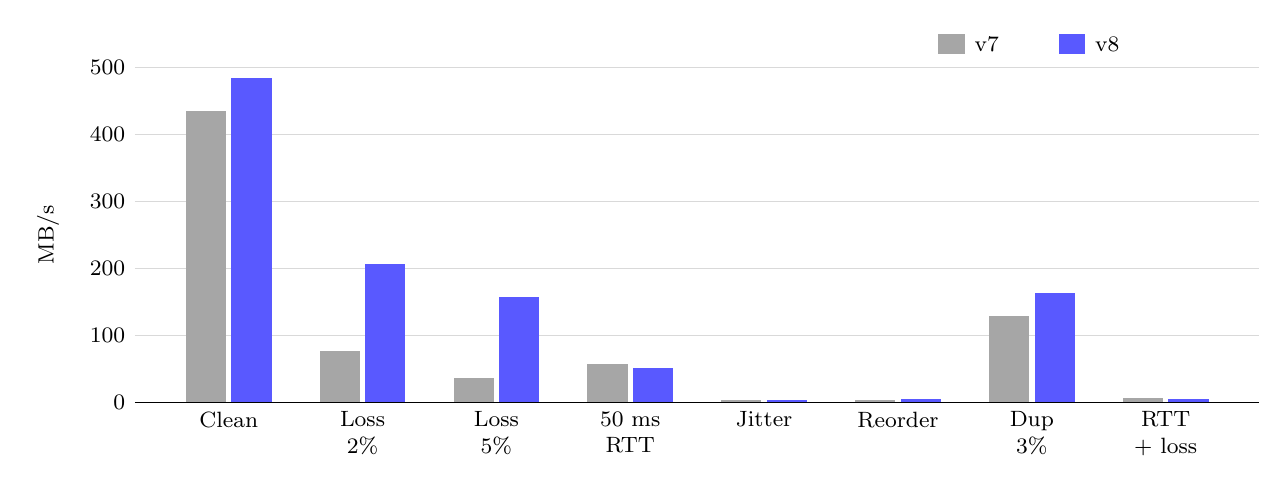
\begin{tikzpicture}[x=1.7cm,y=0.0085cm,font=\footnotesize]
  \foreach \y in {0,100,200,300,400,500} {\draw[black!15] (0.3,\y) -- (8.7,\y); \node[left] at (0.3,\y) {\y};}
  \foreach \i/\n/\a/\b in {1/Clean/435.4/483.6,2/Loss\\2\%/75.6/206.8,3/Loss\\5\%/36.0/157.3,4/50 ms\\RTT/57.5/51.4,
                           5/Jitter/2.7/2.8,6/Reorder/3.8/4.1,7/Dup\\3\%/128.6/163.1,8/RTT\\+ loss/6.8/5.2} {
    \fill[black!35] (\i-0.32,0) rectangle (\i-0.02,\a);
    \fill[blue!65] (\i+0.02,0) rectangle (\i+0.32,\b);
    \node[below,align=center] at (\i,0) {\n};
  }
  \draw (0.3,0) -- (8.7,0);
  \node[rotate=90] at (-0.35,250) {MB/s};
  \fill[black!35] (6.3,520) rectangle ++(0.2,30); \node[right] at (6.5,535) {v7};
  \fill[blue!65] (7.2,520) rectangle ++(0.2,30); \node[right] at (7.4,535) {v8};
\end{tikzpicture}}
\caption{Table~\ref{tab:netem} as a chart. The largest gains are under packet loss.}\label{fig:netem}
\end{figure}

\paragraph{Loss.} Version~8 gains most under loss: 2.7 times faster at 2\% and 4.4 times at 5\%. Selective
acknowledgement stops the resending of blocks the receiver already holds, and the timeout repairs a burst of
known holes at once instead of one block per timeout. The number of retransmissions stays roughly the same
(about 700 at 2\%, 1,700 at 5\%), but they are now the right ones.

\paragraph{Duplication.} Under duplication, version~8 makes no retransmissions at all, against 47 in version~7,
because duplicates no longer disturb the loss signal.

\paragraph{Jitter and reordering.} These are essentially unchanged. Both versions correctly treat a late block
as late rather than lost until the reorder delay expires, and at these settings the relay's own reordering
dominates.

\paragraph{Long delay.} With or without loss, version~8 is 11--24\% slower. This is the intended consequence of
fix~\#8. Version~7's window counted blocks of whatever size they had grown to, so it silently held up to 13
times more bytes than its nominal size. That inflated throughput on a clean long path, but it is unfair to
competing traffic and fragile under loss. Version~8 must earn its window through slow start and additive
increase. On transfers of 32~MiB the window does not reach the path's capacity, while longer transfers amortise
the ramp.

\section{Loopback throughput}

With 512~MiB over four lanes (median of three runs), version~7 reached 1,045~MB/s with 1,644 retransmissions and
version~8 1,079~MB/s with 706 retransmissions. The hardening therefore cost no loopback throughput, even though
every acknowledgement is now processed selectively. Flow control and selective acknowledgement more than halve
the needless retransmissions, which on loopback come from the receiver's rings overflowing, not from the
network.

\section{Earlier comparative benchmarks}

The repository's benchmark record~\cite{repo}, measured during development of versions~5--7 on a 16-core host,
compares Fuse with the quinn QUIC implementation~\cite{quinn}:
\begin{itemize}
  \item \textbf{File transfer.} For a 1~GiB file with both sides encrypted, Fuse reached 3,560~MB/s against
    1,947~MB/s for QUIC at four lanes, 1.8 times faster; unencrypted it was 1.3--2.2 times faster.
  \item \textbf{Latency under load.} Small-message 99th-percentile latency was 39.6~\textmu s alone and
    38.2~\textmu s while 6.3~GB/s of bulk traffic shared the session. A single QUIC connection carrying both
    inflated its tail latency 82 times; a second QUIC connection recovered most of it. This is the clearest
    evidence for per-stream congestion control.
\end{itemize}
These numbers were measured on loopback, with 16~KiB blocks that a 1,500-byte path would not allow, and compare
PSK encryption without forward secrecy against TLS~1.3 with it. They should be read as evidence about
mechanisms, not as predictions for a wide-area network.

\section{Threats to validity}

\begin{itemize}
  \item All measurements are single-host: impairments are emulated by a user-space relay, and no physical
    two-host or real 1,500-MTU path has been measured yet.
  \item Each cell of Table~\ref{tab:netem} is a single run; differences of a few percent are within noise.
  \item The relay itself limits absolute throughput at high rates, although it limits both versions equally.
  \item The comparison with QUIC predates version~8 and has not been repeated since.
\end{itemize}
